% 2_literature-review.tex

\cleardoublepage
\chapter{Literature review}\label{chapter:literature-review}

  This chapter examines the relevant literature associated with the different aspects of the work conducted as part of this thesis. 
  
 
  Explain order of literature and what was examined.
  
  
  \nomenclature[a]{REST}{Rectangular-to-Elliptical Shape Transition}
  
  
  \section{Small Satellite Launchers}
  
  What point do I want to make in this section?
  
  The rocket-scramjet rocket launch system under development at The University of Queensland will face competition from a number of private and public organisations.  
  These organisations are currently developing small satellite launchers to offer bespoke launches with low costs and relatively rapid turn around times. A summary of the small satellite launchers currently in active development is shown in Table \ref{tab:smallsats}. Many of these launchers are projected to be available within the next few years, and will offer cost-per-kg comparable to piggybacking on larger launches. 
  
  Much of the market niche fulfilled by each launch system is determined by the payload to orbit capabilities of the vehicle. Although the launchers shown are all classed as 'small satellite launchers', organisations seeking a launch service will choose a launcher which is designed to launch payloads of comparable size to their desired payoad, for maximum cost efficiency. There is a large variation in the payload-to-orbit capabilities of the small satellite launchers in development, ranging between 50kg to 500kg. The rocket-scramjet-rocket system studied in this thesis will target approximately 150kg of payload to orbit, most similar to the Vector-H\cite{Vector}, Haas2CA\cite{ARCA}, Bloostar\cite{Bloostar}  and Electron\cite{Electron}. 
  
   There are two distinct design method currently employed by small satellite launcher developers; cost efficiency through simplicity, and cost efficiency through reusability. The majority of the small satellite launchers in development are non-reusable. The non-reusable small satellite launch systems aim to reduce costs by creating a launch system which is as cost-efficient as possible to produce and launch. This generally entails making use of conventional, well-tested designs, combined with state of the art manufacturing techniques, such as 3-D printing. This method allows for rapid development, although it has an intrinsic cost limit due to the requirement of manufacturing a new launch system for each launch.  The reusable small satellite launchers aim to reduce costs by virtue of much, or all, of the launch system being able to be used for multiple launches. This method of cost reduction has far higher initial development costs, but has the potential for greater cost savings in the long term. It is notable that the launchers with re-use capabilities are entirely within the early stages of development, with no currently projected completion dates. 
   
   The majority of the small satellite launch systems have projected launch costs between \$20000-\$40000USD/kg. The outlier is the Haas2CA\cite{ARCA}, developed by ARCA, which has the ambitious target of \$10000USD/kg. The Haas2CA is a single stage to orbit launcher, powered by a hydrogen peroxide/kerosene aerospike engine. 

\begin{landscape}% Landscape page
	\begin{table}

  \begin{tabularx}{\linewidth}{|X|X|X|X|X|X|X|X|}
  	
  	\hline  \textbf{Launcher} & \textbf{Company} & \textbf{Country} & \textbf{Payload Capacity} & \textbf{Cost/Kg} (USD) & \textbf{Availability }& \textbf{Stages \& Propulsion} & \textbf{Reusability}  \\ 
  	\hline  Electron \cite{Electron} & RocketLab & NZ/USA & 150Kg to SSO & \$32,600 & Available & Rocket-rocket & No \\ 
  	\hline Lynx \cite{Lynx} &  XCOR & USA & - & - & - & rocket-rocket & First stage \\ 
  	\hline LauncherOne \cite{Virgin} & Virgin Orbit & UK & 300kg to SSO & \$33,000 & - & Aircraft-rocket-rocket & Aircraft\\ 
  	\hline Bloostar \cite{Bloostar} & Zero2Infinity & Spain & 100kg to SSO & \$40,000 &  - & Balloon-rocket-rocket-rocket & No \\ 
  	\hline XS-1 \cite{DARPA2017} & Boeing & USA & - & - &  - & - & First Stage\\ 
  	\hline Eris \cite{Gilmour} & Gilmour Space Technologies & Aus/SG& 380kg to LEO  &\$23,000-38,000   & Q4 2020 && No\\ 
  	\hline Black Arrow 2 \cite{Horizon}& Horizon   & UK & 350kg to SSO & - & 2019 & Rocket-rocket & No \\ 
  	\hline Haas 2CA \cite{ARCA} & ARCA  & USA & 100Kg to LEO & \$10,000 & 2018 & Rocket & No \\ 
  	\hline Intrepid-1 \cite{Intrepid} & Rocket Crafters  & USA & 376kg to SSO & \$23,936 & Q1 2019 & Rocket-rocket & No \\ 
  	\hline KZ-1A \cite{FT1} & CASIC  &  China & 250kg to SSO  & - & - & Rocket-rocket & No \\ 
  	\hline 500R \cite{500R} & Orbital Access  & UK & 500kg to SSO & - & - & Aircraft-Rocket & Fully Reusable \\ 
  	\hline Vector-H \cite{Vector}& Vector Space Systems  & USA & 160kg to LEO  & \$21,875 & 2018 & rocket-rocket-(third rocket optional)& No\\ 
  	\hline SMILE \cite{Kuhn2017} & NLR &  EU & 50kg & $<$\$50,000 & -  & -& -\\ 
  	\hline 
  \end{tabularx} 
  \label{tab:smallsats}
\end{table}
\end{landscape}
\section{Airbreathing Access to Space Systems}


The possibility of using airbreathing stages in access to space systems has been studied in some detail. These systems have been investigated in various forms including; single stage\cite{Powell1991,Wilhite1991,Varvill2008}, dual stage \cite{Tsuchiya2005}\cite{Mehta2001} and tri stage \cite{Preller2017} designs. The most prominent of the airbreathing access to space systems currently in development is the SKYLON Spaceplane being developed by Reaction Engines Limited \cite{Varvill2004}. The SKYLON is a spaceplane which utilises SABRE, a combined cycle airbreathing rocket propulsion system potentially reusable for 200 flights, and is being developed to deliver payloads on the order of 2800kg to heliosynchronous orbit \cite{Sky-rel-ma-}.

\begin{figure}[ht]
	\centering
	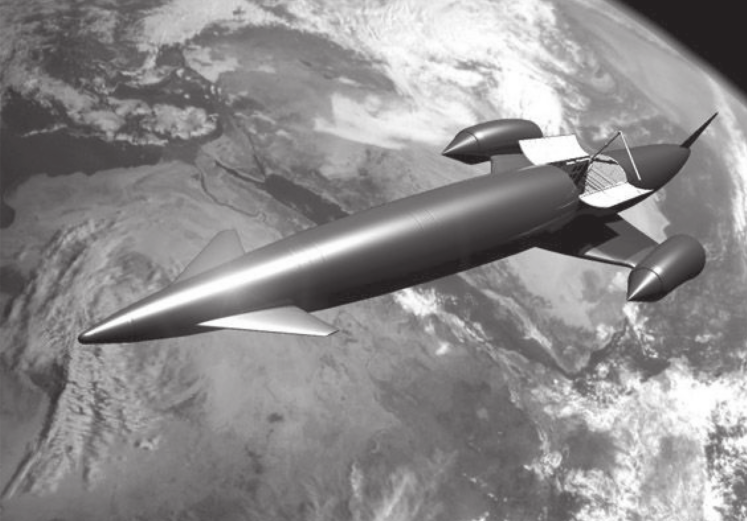
\includegraphics[width=0.6\linewidth]{SKYLON}
	\caption{The SKYLON spaceplane \cite{Varvill2008}.}
	\label{fig:SKYLON}
\end{figure}
A single stage design has the advantage of being fully contained within one vehicle, which is convenient for reusability and return trajectories however is has been suggested by Smart \& Tetlow \cite{Smart2009} that these designs suffer from severe limitations as they must contain multiple engines which add mass at later stages of the trajectory and decrease the efficiency of the vehicle. Smart \& Tetlow suggest that multistage systems offer significant improvements in payload mass fractions, and have the advantage of using airbreathing stages only within their operable range.
Dual stage designs have been investigated in some detail using the 'spaceplane' concept by Mehta \& Bowles \cite{Mehta2001} using life cycle cost analysis in order to take flexibility and reusability into account. Mehta \& Bowles conclude that a two stage design is the optimal configuration for reusable hypersonic space access systems, however this study is only based on comparison with single stage to orbit systems, and it is more useful to consider their conclusions as an endorsement of multi stage airbreathing designs in general. They find that multi stage vehicles have higher potential for payload that single stage to orbit (SSTO) systems and have less propellant requirements, partly due to a greater atmospheric cruise capability. 




\section{Scramjets}



A Scramjet, or supersonic combustion ramjet, is an airbreathing engine design which combusts air at supersonic speeds and is capable of high Mach number operation. Scramjets were proposed in the 1940's \cite{Curran2001} and found to be capable of positive net thrust in 1993 \cite{Paull1993} but have yet to be developed to a level which would allow for commercial application. Scramjet powered vehicles are a potential candidate for small payload delivery systems, offering much higher specific impulse than rockets over their operating range \cite{Billig1993} \cite{Cook2003}. Scramjet engines exhibit this advantage within their operating range due to using atmospheric oxygen for reaction and only carrying fuel, increasing the payload mass that the scramjet vehicle is able to carry. Figure \ref{fig:AirbreathingCorridor} shows the operating corridor for scramjet engines, indicating the point at which transition to rocket stage would occur, the lower dynamic pressure limit on engine operation and the upper dynamic pressure limit on the aircraft structure.
\begin{figure}[ht]
	\centering
	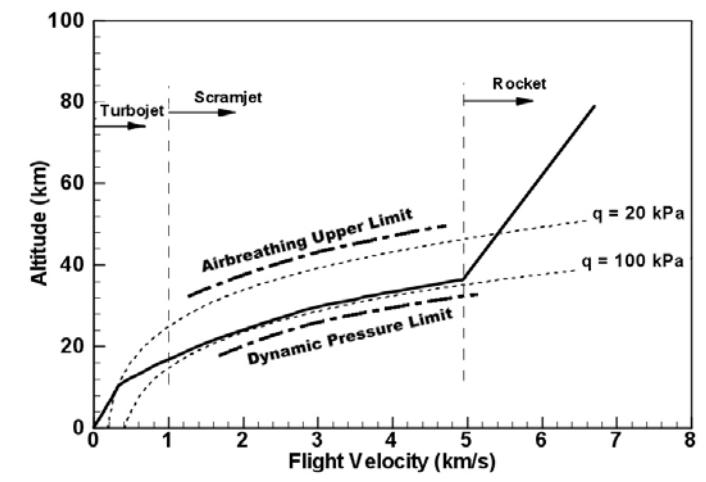
\includegraphics[width=0.7\linewidth]{AirbreathingCorridor}
	\caption{The airbreathing vehicle flight corridor \cite{Smart2010}.}
	\label{fig:AirbreathingCorridor}
\end{figure}

Smart \& Tetlow \cite{Smart2009} have found that the fuel savings achieved by using a scramjet engine within these limits, coupled with small necessary payload mass, may enable the development of a partially or fully reusable space access system utilising a scramjet powered stage in the near future. Simulations carried out  for three stage systems utilising scramjet and rocket engines for small payload delivery show favourable payload mass fractions with a reusable scramjet stage  \cite{Smart2009}. Scramjet powered vehicles may also offer the ability to put small payloads into orbit with greatly increased flexibility and launch window when compared to similarly sized rocket systems. This has been assessed in a study by Flaherty  \cite{Flaherty2010} comparing the United States Air Force's Reusable Military Launch System all-rocket launch vehicle RMLS102 against the Alliant Techsystems rocket/scramjet launch system ATK-RBCC. These vehicles are similarly sized and comparisons were made for payloads launched to rendezvous with satellites in randomly generated orbits. These vehicles were compared using the range of orbital trajectories that each vehicle was able to rendezvous with within one day, determined by launch vehicle range. The rocket/scramjet ATK-RBCC was found to have a large advantage in trajectory flexibility over the rocket only vehicle, in a large part due to the scramjets ability to fly fuel efficiently over long distances. This means in general that a partially scramjet powered accelerator  is able to fulfil the specific delivery needs of small payloads over a wider range of orbits within smaller time periods when compared to a fully rocket powered accelerator. This can be advantageous for time critical and orbit dependant payloads which have specific mission requirements to be met. 




\section{The SPARTAN}





The three stage, partially reusable, access to space system under development at The University of Queensland utilises the SPARTAN\cite{Jazra2013} scramjet powered vehicle as the reusable second stage, shown in Figure \ref{fig:SPARTAN}. This system is considered in this study as a representative model for three stage, airbreathing access to space system designs. This launch system is designed for small payload deliveries to orbit and will in the future utilise a fly-back rocket booster to accelerate the SPARTAN stage to minimum Mach number required for stable burn, at which point separation occurs and the second stage uses a scramjet engine to accelerate to between approximately Mach 5-9. The first and second stages are to be reusable, the first stage via conversion into a propeller powered drone, and the second stage through either a glide or extra scramjet powered flight to a suitable landing site. However, the first stage booster considered in this study is a simple disposable design. The ascent profile is of interest to this study, however development of the fly-back trajectory profile requires detailed first stage vehicle design which is outside of the scope of this study. 

\begin{figure}[ht]
	\centering
	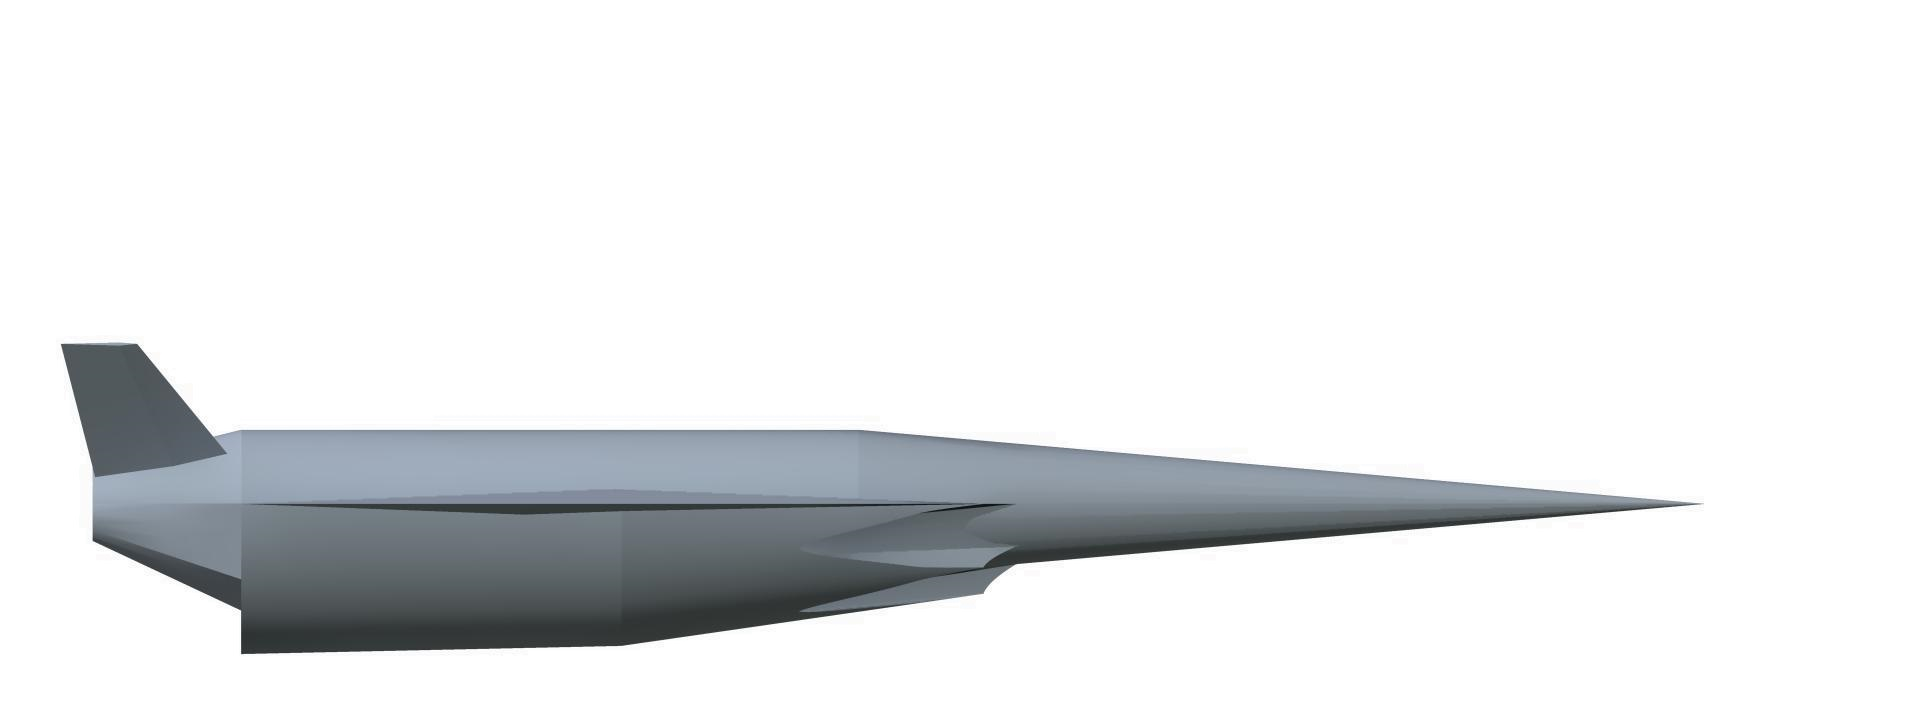
\includegraphics[width=0.7\linewidth]{SPARTAN}
	\caption{An early design of the socket-scramjet-rocket launch system incorporating the SPARTAN \cite{Jazra2013}.}
	\label{fig:SPARTAN}
\end{figure}

The third stage will be a disposable rocket stage, which will then deliver the payload to orbit, exiting the atmosphere and performing a Hohmann transfer. 

This system is in the preliminary design stage, with estimates of  payload mass fraction indicating that 1.26\% PMF is possible when delivering a 257.4kg payload to low earth orbit \cite{Preller2015a}. This compares well with existing space systems of similar size, with the advantage of being designed for reusability. The second stage vehicle has been designed to a detailed level, and optimised for payload delivery to heliosynchronous orbit.

The SPARTAN has been studied in some detail, simulated over a constant dynamic pressure trajectory with variation in the aerodynamic surface properties of the vehicle. 

\subsection{Scramjet Engine Model}
To deliver a payload to orbit, the SPARTAN uses four Rectangular-to-Elliptical Shape Transition (REST) scramjet engines, with inlets configured to allow installation on a conical forebody. This study uses engines configured to fly between Mach 5 and 10, this type of engine is known as a C-RESTM10 engine\cite{Preller2017}. The REST model has been studied experimentally for flight at off design conditions by Smart \& Ruf \cite{Smart2006}. The REST engine has been used as it has been proven to operate successfully at off-design conditions, an extremely important property for this study as the scramjet stage experiences a range of Mach number flight conditions, and significant variation in dynamic pressure.  

A propulsion database of the C-RESTM10 has been provided for this study by Prof. Michael Smart.
\begin{figure}
\centering
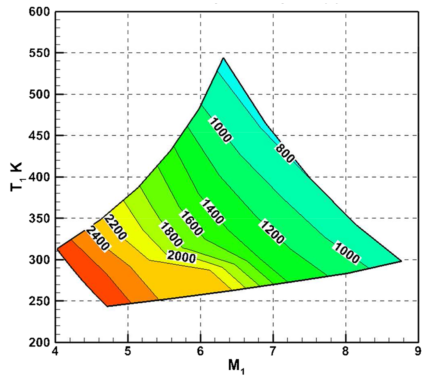
\includegraphics[width=0.7\linewidth]{figures/2_literature-review/C-REST}
\caption{The C-RESTM10 propulsion database, specific impulse.}
\label{fig:C-REST}
\end{figure}



\section{First Stage Rocket Booster}

The SPARTAN scramjet vehicle must be accelerated to its minimum operating speed by a first stage rocket booster. This booster must be capable of efficient operation from launch at sea level until staging. It is envisioned that the SPARTAN system will eventually use a reusable flyback booster\cite{Preller2017}. However the flyback of the first stage is outside the scope of this study. Instead, a model of an existing first stage booster will be used, for which the Falcon-1e was chosen.

The SpaceX Falcon-1e launch system was a proposed small satellite launch system which would have entered use after 2010\cite{Vehicle2008}, but was discontinued and superseded by the Falcon-9 project. The Falcon-1e was designed to launch payloads between 600-900kg to low Earth orbit, with flexible orbit altitude and inclination. The Falcon-1e was to be the next generation of the Falcon-1\cite{Vehicle2008}, a launch tested, modern launch system. The Falcon-1e was chosen for its appropriate size and the proven flight effectiveness of the Falcon-1. The first stage of the Falcon-1e is powered by a Merlin 1C LOX/Kerosene turbopump engine. The first stage rocket is designed to be a Falcon-1e first stage scaled lengthwise to 50\% of its original length. 


\section{Exoatmospheric Rocket Engines}
After scramjet stage burnout, the upper stage rocket must exit the atmosphere, and accelerate the payload to orbital velocity. This requires a rocket engine with sufficient thrust to accelerate the third stage rocket out of the atmosphere, and a diameter small enough to allow the rocket to fit within the fuselage of the SPARTAN. Table \ref{tab:Engine} shows a comparison study of upper stage rocket engines. 

\begin{landscape}% Landscape page
\begin{table}

\begin{tabularx}{\linewidth}{|X|X|X|X|X|X|X|X|X|}

	\hline Engine & Fuel Supply & Fuel & Thrust & Isp & Mass & Diameter & Length & Thrust Vector Capability \\ 
	\hline Aestus & Pressure-fed & MMH/NTO & 27.5kN & 320s & 110kg & 1.27m & 2.2m & 4$^\circ$ \& 4$^\circ$ by mechanical adjustment\\ 
	\hline OMS & Pressure-fed  & MMH/NTO & 26.7kN & 316s & 118kg & 1.168m & 1.956m & 8$^\circ$\\ 
	\hline Aestus II & Pump-fed & MMH/NTO & 46kN & 337.5s & 148 &  & 2.2m  & 6$^\circ$\\ 
	\hline RS-72 & Pump-fed & MMH/NTO & 55.4kN & 338s & 154kg &  & 2.286 &  6$^\circ$\\ 
	\hline ATE & Pump-fed & MMH/NTO & 20kN & 345s & 57.9kg & 0.38m & 1.4m &  15$^\circ$\\ 
	\hline AJ10-118K & Pressure-fed & A-50/NTO & 43.3kN & 320.5s & 124.5kg & 1.53m & 2.7m & Fixed \\ 
	\hline Kestrel & Pressure-fed & LOX/Kerosene & 30.7kN & 317 & 52kg & 1.1m & 1.9m  & Yes, Unknown limits\\ 
	\hline Rl-10-3A &  &  &  &  &  &  &   &\\ 
	\hline  &  &  &  &  &  &  &  & \\ 
	\hline 
\end{tabularx} 
\caption {Comparison of upper stage rocket engines.} 
\label{tab:Engine}
\end{table}
\end{landscape}


\section{Partially-Airbreathing Launch Vehicle Ascent Trajectories}

Current simulations of the SPARTAN vehicle have been carried out with the assumption of a 50kpa dynamic pressure trajectory, a likely design point of the vehicle and scramjet engine. 
 Constant dynamic pressure trajectories have been used for airbreathing vehicle simulation due to the trade-off between structural loading and engine performance for hypersonic vehicles \cite{Olds1998} . As dynamic pressure increases so does the structural loading on the vehicle, however scramjet thrust is directly reliant on dynamic pressure ie. an increase in dynamic pressure directly means more air into the engine inlet. A constant dynamic pressure is viewed as being an acceptable compromise between these two factors.   
This form of trajectory has so far been simulated using proportional integral derivative (PID) feedback control, directly investigated since 1998 by Olds \& Budianto \cite{Olds1998}. This is a simple and effective form of control for systems being simulated over a constant dynamic pressure path \cite{Preller2015}. This form of control utilises minimises an error function as the vehicle moves along its trajectory. This error function causes the controls of the vehicle to be modified by a feedback term which is a function of the error including proportional, integral and derivative terms. The result is a trajectory which is suitably close to the objective design point, with minimal overshoot and steady state error which can cause oscillations around the specified design value. Figure \ref{fig:PID} shows an example of a constant gain PID controller as applied to the SPARTAN vehicle being simulated to a design point of 50kPa dynamic pressure. Oscillations can be observed around the design point due to overshoot and steady state error, factors which are prevalent in PID control systems.

\begin{figure}[ht]
	\centering
	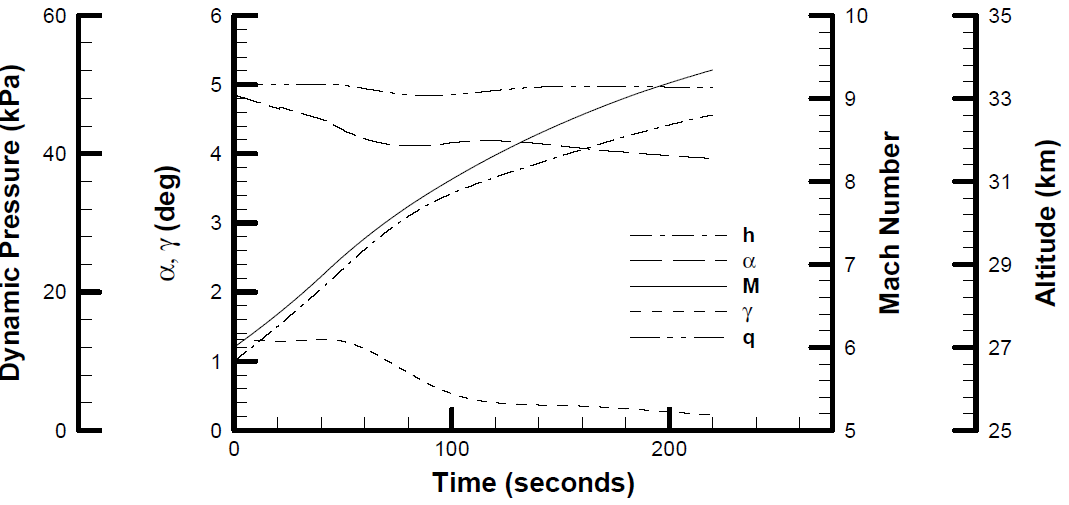
\includegraphics[width=0.9\linewidth]{PID}
	\caption{An example of a constant gain PID controller, controlling the SPARTAN trajectory around a 50kPa dynamic pressure design point \cite{Preller2015}.}
	\label{fig:PID}
\end{figure}


It is possible that a constant dynamic pressure trajectory may not be the most appropriate trajectory for the second stage vehicle, as there is a variety of aerodynamic factors that must be considered in designing optimal payload to orbit flight. It may be optimal for the vehicle to fly at less than maximum dynamic pressure at point throughout the trajectory, most likely at the first to second and second to third stage separation points. For a constant dynamic pressure trajectory the second-third stage transition will occur at a very low trajectory angle. This is suboptimal for the third stage rocket, which needs to perform a large pull up manoeuvre at high dynamic pressure. Launching this system at higher angle or altitude may improve third stage fuel usage greatly, at a small cost to the second stage fuel, allowing a greater payload to be delivered to orbit. 

\subsection{Single-Stage Vehicles}

Optimal trajectories have previously been developed for launch systems integrating airbreathing and rocket propulsion within single-stage-to-orbit (SSTO) vehicles \cite{Powell1991,Lu1993,Trefny1999}. These optimal trajectory studies found unanimously that a pull-up manoeuvre before the end of the airbreathing engine cut-off was the optimal flight path for the SSTO airbreathing-rocket vehicles being investigated. A pull-up was found to be optimal for vehicles where the rocket engines are not ignited until circularization altitude \cite{Powell1991,Lu1993} as well as vehicles where the rocket engine is ignited immediately after airbreathing engine cut-off \cite{Trefny1999}. For SSTO vehicles a pull-up manoeuvre is a simple trade-off between the altitude at airbreathing engine cut-off and the velocity achievable at cut-off. Due to the entire vehicle being lifted into orbit, this becomes a relatively simple problem of engine efficiency. The airbreathing engine is used for its high efficiency, until the dynamic pressure drops below the operable limit of the airbreathing engine, or until the thrust provided by the airbreathing engine is significantly counteracted by the effects of drag and gravity. 
\begin{figure}[h]
	\centering
	\begin{minipage}[b]{0.3\textwidth}
		\centering
		\includegraphics[width=\linewidth]{"figures/2_literature-review/Powell Vehicle"}
		\caption{}
		\label{fig:PowellVehicle}
	\end{minipage}	
	\begin{minipage}[b]{0.6\textwidth}
		\includegraphics[width=\linewidth]{"figures/2_literature-review/Powell Trajectory"}
		\caption{Powell}
		\label{fig:PowellTrajectory}
	\end{minipage}
	
\end{figure}
 
 \subsection{Multi-Stage Vehicles}

For a multi-stage to orbit vehicle, calculating the optimal trajectory for maximum payload flight is significantly more difficult. A multi-stage vehicle has one or more stage transition points, where the vehicle separates a component which is discarded or reused later, and does not continue to orbit. At a stage transition point there is a large change in the mass and aerodynamics of the launch system. 
This change in flight dynamics makes finding the optimal stage transition point more complicated. To find the optimal separation point there is a trade-off between:
 \rom{1}. The high efficiency of the scramjet engines,
 \rom{2}. The thrust produced by the scramjet engines, 
 \rom{3}. The potential thrust of the rocket engines,
 \rom{4}. The energy necessary to increase the altitude of the scramjet stage,
 \rom{5}. The aerodynamic efficiency when performing the required direction change.
All of these factors must be considered in order to generate an optimal trajectory. 

There has been a number of studies which have identified a pull-up manoeuvre as being advantageous for a multi-stage system \cite{Tsuchiya2005,Wilhite1991,Mehta2001}. However, in these studies a pull-up manoeuvre has been specified in order to decrease the dynamic pressure of the vehicle at airbreathing-rocket stage separation. 
\begin{figure}
\centering
\begin{minipage}[b]{0.45\textwidth}
	\centering
	\includegraphics[width=\linewidth]{"figures/2_literature-review/Wilhite Booster Vehicle"}
	\caption{}
	\label{fig:WilhiteVehicle}
\end{minipage}	
\begin{minipage}[b]{0.45\textwidth}
\includegraphics[width=\linewidth]{"figures/2_literature-review/WilHite Booster Trajectory"}
\caption{Wilhite}
\label{fig:WilHiteTrajectory}
\end{minipage}
\end{figure}
\begin{figure}
	\centering
	\begin{minipage}[b]{0.45\textwidth}
		\centering
		\includegraphics[width=\linewidth]{"figures/2_literature-review/Tsuchiya Vehicles"}
		\caption{a) Airbreathing b) Airbreathing/Rocket}
		\label{fig:TsuchiyaVehicle}
	\end{minipage}	
	\begin{minipage}[b]{0.45\textwidth}
		\includegraphics[width=\linewidth]{"figures/2_literature-review/Tsuchiya"}
		\caption{The trajectory of the launch system developed by Tsuchiya and Mori \cite{Tsuchiya2005}}
		\label{fig:TsuchiyaTrajectory}
	\end{minipage}
\end{figure}


In the studies by Tsuchiya et al.\cite{Tsuchiya2005} and Wilhite et al.\cite{Wilhite1991}, decreased dynamic pressure is necessary for the successful operation of the orbital rocket stages, of the systems under investigation. In these studies the airbreathing stages pull-up to the maximum allowable dynamic pressure for the rocket-powered orbital stages. When the orbital stages are able to operate, stage separation occurs. These pull-up manoeuvres demonstrate the advantages of a pull-up for the operation of the orbital stages, allowing the aerodynamic and thermal loading on the vehicle to be reduced. However these pull-up manoeuvres are not performed as part of optimal trajectories, instead they are designed to ensure that the performance constraints of the systems are met. 

\begin{figure}
	\centering
	\begin{minipage}[b]{0.3\textwidth}
		\centering
		\includegraphics[width=\linewidth]{"figures/2_literature-review/Mehta Vehicle"}
		\caption{}
		\label{fig:MehtaVehicle}
	\end{minipage}	
	\begin{minipage}[b]{0.6\textwidth}
		\includegraphics[width=\linewidth]{"figures/2_literature-review/Mehta Trajectory"}
		\caption{The trajectory of the launch system developed by Mehta and Bowles \cite{Mehta2001}.}
		\label{fig:MehtaTrajectory}
	\end{minipage}
	
\end{figure}
Mehta \& Bowles \cite{Mehta2001} prescribe a 2g pull-up at flight conditions of Mach 10, 95000 ft for an airbreathing stage in order to "lower dynamic pressures and to achieve the optimal launching flight path angle for the orbiter vehicle". This indicates that a pull-up manoeuvre before airbreathing-rocket transition is considered the optimal trajectory, however this study does not optimise the shape or magnitude of the pull-up manoeuvre, only considering the increased performance of the rocket vehicle. 



\section{Hypersonic Vehicle Flyback Trajectories}

Past studies of the SPARTAN vehicle have assumed that a fly-back to launch site is possible after third stage separation\cite{Preller2017}. However, this fly-back has not yet been simulated. A simulation of the fly-back of the SPARTAN is necessary in order to assess the viability of the SPARTAN concept.
The fly-back of the SPARTAN is a crucial component to the viability of the rocket-scramjet-rocket launch system. The SPARTAN must return to the initial launch site to enable refurbishment to begin immediately, and so that there is no significant transportation of the SPARTAN required between launches. 
Due to the second-third stage staging velocity, it is complicated for the SPARTAN to cover the necessary fly-back distance. 
To maximise fuel efficiency, it is desirable for the SPARTAN to perform a minimum-fuel fly-back to the initial launch site, with the best-case scenario being for the fly-back to use no fuel at all.

There are three main methods that have been studied for potential hypersonic vehicle return; glide-back, cruise-back and boost-back. Glide-back involves the hypersonic vehicle returning to base and landing entirely using its aerodynamics. This requires sufficient lift to sustain the hypersonic vehicle over the entire return range, as well as the controllability to land the hypersonic vehicle in level flight. 
For a hypersonic trajectory a fully glide-back return flight is most likely unobtainable. This is due to the large downrange distance flown, and the large initial velocity at the beginning of the fly-back trajectory, when the vehicle is oriented away from the landing site. Multiple studies have investigated the maximum staging velocity allowable for the glide-back flight of a booster. 
In these studies, the maximum separation velocity for glide-back to be feasible has been found to be between Mach 3-4 at 30km-120km downrange distance, with higher initial velocities or longer downrange distances requiring fly-back under power\cite{Hellman,Tetlow1992}.

Cruise-back involves the inclusion of subsonic engines, which are used to power the fly-back of the hypersonic vehicle until landing similar to a conventional aircraft. These engines may be included solely for the fly-back\cite{Hellman}, or used in the acceleration phase for low velocity acceleration\cite{Mehta2001,Tetlow1992,Wilhite1991}. The addition of subsonic engines powering a constant velocity cruise-back phase allows the accelerator to return to base with a similar trajectory to that of traditional aircraft, allowing the velocity and altitude of the accelerator to be precisely controlled. However, the addition of subsonic engines necessary for cruise-back increases the mass of the vehicle significantly, leading to decreased mass efficiency and increased design complexity\cite{Hellman}. 

A preferable mode of powered fly-back is to use the existing hypersonic airbreathing engines during the return trajectory in a boost-back trajectory. Using the existing airbreathing engines allows for range to be added to the return trajectory, without the inclusion of additional engines. The hypersonic airbreathing engines can be operated at appropriate times during the fly-back, when they will be most impactful on the return trajectory range. However, the hypersonic airbreathing engines may only be used within their operating region, and vary in thrust and efficiency dependent on flight conditions. Hypersonic airbreathing engines have maximum efficiency at low Mach numbers\cite{Preller2017}, with the thrust produced depending on the dynamic pressure and inlet conditions, which vary with the trajectory path and angle of attack of the vehicle. This added complexity requires the use of trajectory optimisation methods to find the most efficient flight path for return to the launch site, and to ensure that the return of the vehicle under its own power is viable. 

\subsection{Examples of Optimised Fly-Back Trajectories}

Tetlow et al. \cite{Tetlow1992} compare powered cruise-back to glide-back flight for the return of the first stage booster of a rocket powered two-stage launch vehicle. The powered flyback vehicle uses airbreathing engines to cruise back to the launch site at relatively low speeds. The powered flyback and the glide-back cases are analysed separately to determine the difference in the optimal staging velocities. Figure 2 shows the optimised deceleration phase for the cruise-back vehicle, terminating at cruise-back conditions. This trajectory shows three distinct ‘skips’, with the minimum trajectory angle progressively decreasing between each. Tetlow et al. conclude that the 'skips' are due to the rate of density increase being greater than the deceleration rate 'causing increased lift and levelling out of the altitude profile'\cite{Tetlow1992}. This trajectory was optimised for minimum cruise-back fuel mass, indicating that the 'skips' are the optimal trajectory shape to maximise range in high initial velocity fly-back. The powered cruise-back vehicle is able to stage at 3000m/s due to the ability to cover a large distance during cruise-back. 
The glide-back vehicle was optimised to find the maximum possible staging velocity at which a turn and glide-back is still possible. This was found to be at 1200m/. Figure 3 shows the corresponding optimal deceleration trajectory, terminating at sustainable glide conditions. This trajectory again shows multiple ‘skips’. The low allowable separation velocity of 1200m/s for the glide-back booster potentially suggests that the SPARTAN will require powered flyback. 
Tetlow et al. assume an admittedly optimistic L/D of 7 at Mach 0.9, and maximum angle of attack of 40 deg. However, the mass of the vehicle in this study is up to 1182 tons. A lower L/D may be acceptable for a lighter vehicle.  

A maximum staging velocity at which glide-back is possible is also investigated by Hellman \cite{Hellman}. Hellman uses a suboptimal, scheduled trajectory simulation to investigate the flyback capabilities of a reusable rocket booster. Hellman finds that Mach 3 is the upper staging limit for a glide-back booster. This agrees with Tetlow et al. that high staging velocities are not possible for glide-back boosters, suggesting that the SPARTAN will require powered return flight.

\begin{figure}
\centering
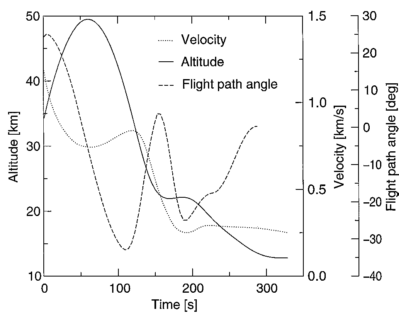
\includegraphics[width=0.7\linewidth]{../../../Dropbox/phd/flyback/Glideback}
\caption{The flight path of a glide-back booster, developed by Tetlow et al. CITEXX.}
\label{fig:Glideback}
\end{figure}

\begin{figure}
\centering
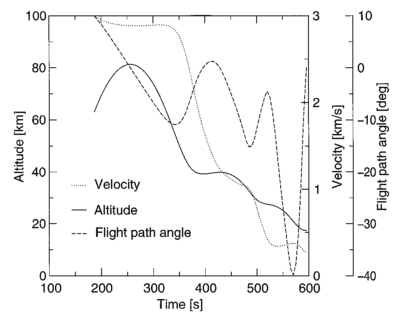
\includegraphics[width=0.7\linewidth]{../../../Dropbox/phd/flyback/Powered}
\caption{The flight path of a powered fly-back booster, developed by Tetlow et al. CITEXX.}
\label{fig:Powered}
\end{figure}


The possibility of an airbreathing vehicle reigniting high speed airbreathing engines for short periods has been investigated by Tsuchiya and Mori \cite{Tsuchiya2005}.  Tsuchiya and Mori investigate two conceptual launch vehicles; a vehicle powered solely by airbreathing propulsion returning after separation of an orbital stage at Mach 5.1, and an airbreathing/rocket vehicle returning after a separation at Mach 6.8\cite{Tsuchiya2005}.  For the purposes of fly-back these vehicles are very similar, both using the high speed airbreathing engines during return flight. The optimal launch and return trajectories for these vehicles are shown in Figure \ref{fig:TsuchiyaTrajectory}. The separation for the airbreathing vehicle occurs at Mach 5.1, and the separation for the airbreathing/rocket vehicle at Mach 6.8. Both optimised return trajectories follow a relatively similar path. A long ‘skip’ is performed, with both vehicles hitting the dynamic pressure limit. Both vehicles ignite the airbreathing engines at around Mach 3.5 for “several tens of seconds” to extend the range of the fly-back manoeuvres. After this, the vehicles descend and land at the launch site. The velocity at the landing point is not constrained, causing the airbreathing vehicle to land at slightly under Mach 1, and the airbreathing-rocket vehicle to land at approximately Mach 0.5. The latter is comparable with the landing velocity of the space shuttle \cite{Romere1983}. 
These boosters fly to a downrange distance of 600-625km from the launch site, and separate from the orbital accelerator at a dynamic pressure of 15kPa\cite{Tsuchiya2005}. At the start of their respective return trajectories, both boosters turn with a bank angle of 130-145$^\circ$. Both the fully-airbreathing and partially-airbreathing vehicles ignite their airbreathing engines for 'several tens of seconds' at approximately Mach 3.5, in order to extend the flight range of the vehicles and return to the initial launch site\cite{Tsuchiya2005}. Less than 5\% of the vehicles initial propellant was required to return the vehicles to the initial launch sites\cite{Tsuchiya2005}.

These optimised return trajectories show three distinct sections; a turn manoeuvre, a skipping phase, and a high L/D descent. The skipping phase is similar to the boost-skip trajectory of the space shuttle CITEXX, which uses repeated entries into the atmosphere, and skips out, to extend the range of an atmospheric entry. A skipping trajectory has been shown to be range optimal for hypersonic vehicles able to skip out of the atmosphere \cite{Moshman2014}, as well as vehicles flying entirely within the atmosphere\cite{Moshman2014,Darby2011}. A skipping trajectory has also been shown to be optimal for an air-breathing hypersonic vehicle thrusting throughout the trajectory\cite{Chai2015}. The range optimal operation of the air breathing engine is shown to be repeated ignitions at the trough of each skip. The scramjets are ignited as the vehicle climbs after the through, as the Mach number decreases to the minimum operable conditions of the scramjet engines. Minimising the Mach number during operation in this way maximises the efficiency of the scramjet engines.

\begin{figure}
\centering
\includegraphics[width=0.9\linewidth]{"figures/2_literature-review/chai-boost skip"}
\caption{}
\label{fig:chai-boostskip}
\end{figure}


When compared to the vehicles investigated by Tsuchiya and Mori\cite{Tsuchiya2005}, the SPARTAN separates from its third stage rocket at a considerably higher Mach number of Mach 9.1, as well as at a considerably higher dynamic pressure of 33.9kPa. The SPARTAN must also cover a longer fly-back range of 878km. In addition, the C-REST scramjet engines are limited to operating at hypersonic speeds of Mach 5.1 or higher. These design differences create substantially more challenging conditions than those studied by Tsuchiya and Mori. Consequently, it is necessary to investigate the ability of the SPARTAN to return to the launch site following separation. From comparisons of the studies within this section it is evident that an optimisation of the return flight of the SPARTAN is required, and that a simply defined trajectory is not appropriate.

\section{Optimal Control}


To this point analysis of the SPARTAN trajectory has been performed using PID feedback control, assuming a constant dynamic pressure trajectory \cite{Preller2015}. PID feedback control simulates the vehicle flight and manoeuvres the vehicle so that the trajectory conforms to a defined design point. Currently the trajectory of the SPARTAN has been simulated to align as closely as possible with 50kPa flight, a problem for which PID control is well suited. 

This study aims to find the optimal trajectory path for the SPARTAN that will produce maximum payload to orbit capability for the three stage system. Feedback control is infeasible for finding an optimal trajectory shape as there is no single design point at each stage of the simulated trajectory to calibrate towards. A control method is required that can take into account all aerodynamic factors at every timestep in order to find an optimal trajectory. Defining the trajectory simulation as an optimisation problem allows the trajectory to be solved at every point simultaneously, producing an optimal trajectory over the entire simulation space. Optimal control theory is widely used in situations where an optimal trajectory path must be found, and has been used widely in aerospace applications. However a trajectory optimisation has not been attempted on a three stage airbreathing system, and is usually reserved for simpler systems as there can be issues with convergence and long computation times \cite{Diehl2006}. This does not rule out using an optimisation method on a complex aerodynamic system however it does reinforce that choosing the correct optimisation procedure and defining the problem in the correct way is integral to developing an accurate solution method. This study aims to find a method of optimisation that is applicable to a complex aerodynamic trajectory and to apply this to the SPARTAN vehicle to produce an optimal trajectory shape for maximum payload delivery to heliocentric orbit.

For an optimisation of a complex trajectory there are a variety of optimal control methods that are useful for specific problem types. These are separated into two categories: direct and indirect solution methods. Indirect methods are based on the calculus of variations or minimum principle model, and generally result in high accuracy solutions to optimisation problems \cite{Bulirsch1993}. However indirect models suffer from the drawbacks of small radii of convergence and the fact that the equations to be solved often exhibit strong nonlinearity and discontinuities. This means that indirect methods will not be solvable unless the problem is very well defined with a minimum of nonlinearity, making indirect methods unsuitable for many complex optimisation problems such as aerospace vehicle simulations which can exhibit strong nonlinear behaviour and have a wide solution space. 

Direct methods transform an optimisation problem into a nonlinear programming (NLP) problem which can be solved computationally \cite{Stryk1992}. NLP solvers solve the optimisation problem defined as \cite{Bazaraa2013}:

\begin{equation}
Minimise \qquad f(x)
\end{equation}

\begin{equation}
Subject \quad to \qquad g_i(x)\leq0 \quad for \quad i=1,...,m
\end{equation}

\begin{equation}
and \qquad h_j(x) = 0 \quad for \quad j=1,...,n
\end{equation}

An optimisation problem that has been discretised in this form can thus be solved using any of a variety of NLP solvers. One of the most effective methods of solving twice differentiable NLP problems is sequential quadratic programming (SQP) \cite{Boggs2000} for which there is a variety of commercial solvers available such as NPSOL, SNOPT and packages within MATLAB. 

In order for these packages to be able to solve an optimisation problem it must be presented in discretised form, and as such must be transformed using approximation techniques. The task of approximating a continuous optimisation problem in discrete NLP solvable form is not simple. SQP solvers can very easily run into convergence issues when provided with an optimisation problem which has not been well defined over a logical solution space. Also, any approximation must be carried out with care that the accuracy of the solution is not compromised. There are multiple ways to approximate a continuous optimisation problem directly as an NLP problem, the most common of which are shooting and collocation methods. The differences in the behaviour of each method are related to the interaction between the SQP solver and the discretisation method by which the problem is defined, and can affect the stability and accuracy of the solution as well as the solution time of the problem. For this study of in atmosphere trajectory optimisation with complex atmospheric and vehicle properties it was desired that a method be found with maximum stability and accuracy for a relatively large solution space, while solution time is a secondary priority.

\subsection{The Single Shooting Method}


The oldest and simplest method of approximating continuous optimisation problems as NLP problems is the direct single shooting method. Direct single shooting discretises the control function over the solution space, and solves this directly as an NLP by integrating the vehicle dynamics, or state variables, along the trajectory at each trajectory guess. Single shooting is simple to apply and has been used since the 1970s for rocket trajectory optimisation \cite{jezewski1971}. Single shooting methods suffer from nonlinearity problems, ie. an optimisation problem solved using the single shooting method will potentially struggle to solve if the problem exhibits even small nonlinearities, due to being unable to converge to an optimal solution. This makes the single shooting method unsuitable for complex problems such as a scramjet model, as there are many nonlinear factors inherent in atmosphere and airbreathing engine modelling. 
\subsection{The Multiple Shooting Method}



Direct multiple shooting is a popular solution to trajectory optimisation problems. This method solves some of the instabilities of the single shooting method by splitting the trajectory into multiple shooting arcs, and collocating these at specific time points. This creates a system of discontinuities, illustrated in Figure \ref{fig:multipleshooting}, which are gradually removed by the solver algorithm until the trajectory is continuous. These discontinuities allow greater flexibility for the solver than is afforded by the single shooting method. The multiple shooting problem is solved as an NLP through discretisation of the state and control variables at each time node and integration for the state variables $x$ over each shooting arc $t_k$ \cite{Subchan2008}:
\begin{equation}
\dot{x} = v = f[x(t),u(t)]
\end{equation}
With the state variables subject to the boundary conditions:
\begin{equation}
\qquad r[x(t_0),x(t_f)] = 0
\end{equation}
And solving for the unknown values $s_i$:

\begin{equation}
x(t_i) = s_i, \qquad i = 1,2...N
\end{equation}
The control variables at the nodes are guessed and the state variables are integrated along the trajectory, with each node segment being considered separately. A matching condition is introduced that must be met between each segment; ie. the trajectory must be continuous. \cite{Michalik2009}

\begin{equation}
\textbf{X(s)} = \begin{Bmatrix}
x(t_1;s_0,v_0) - s_1 \\
x(t_2;s_1,v_1) - s_2  \\
\vdots    \\
x(t_N;s_{N-1},v_{N-1}) - s_N  \\
r[x(s_0),x(s_N)]
\end{Bmatrix} = \textbf{0}
\end{equation}
This is now in the form of an NLP problem which may be solved in a standard NLP solver. ie. minimise:

\begin{equation}
\min J(s,v) = \sum_{i=0}^{N-1}J_i(s_i,v_i)
\end{equation}
subject to:
\begin{equation}
x[t_{i+1},s_i,v_i] - s_{i+1} = 0
\end{equation}

\begin{equation}
r[x(s_0),x(s_N)] = 0
\end{equation}



\begin{figure}[ht]
	\centering
	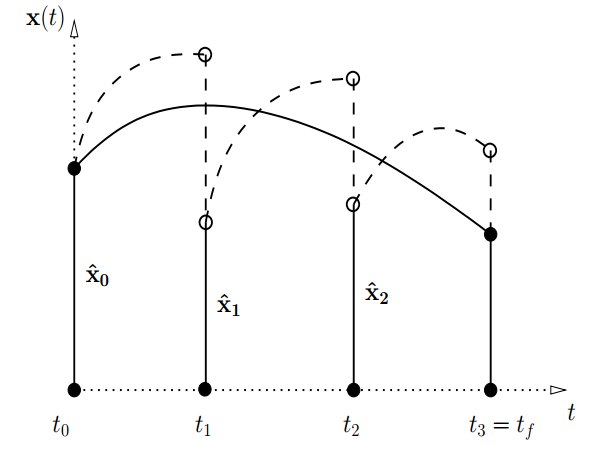
\includegraphics[width=0.7\linewidth]{multipleshooting}
	\caption{An illustration of the subdivision associated with multiple shooting \cite{Michalik2009}. Dashed lines illustrate the initial trajectory guess and the solid line indicates the final trajectory once the joining conditions are met.}
	\label{fig:multipleshooting}
\end{figure}

The multiple shooting method has greatly improved convergence compared to the single shooting method, removing much of the susceptibility to instabilities resulting from nonlinear effects. However, the multiple shooting approach still suffers from a relatively small radius of convergence and slow computation times. Radius of convergence is extremely important to this study as the optimal solution cannot be approximated to a great degree of accuracy, and as such multiple shooting was deemed inappropriate for this study. It was desired to find a method with a global radius of convergence to apply to the optimisation problem being considered.

\subsection{The Pseudospectral Method}\label{sec:PS}

check some of my claims about the pseudospectral method and cite GPOPS papers

GPOPS USES HP-ADAPTIVE GAUSS, WHICH HAS BEEN SHOWN TO improve(?) GAUSS

I should show the hp-adaptive gaussian method

Direct Trajectory Optimization and
Costate Estimation via an Orthogonal
Collocation Method - benson
is quite a good paper (the first?) explaining gaussian ps method

also look at gpops 1 manual

The most promising method found to address the issue of radius of convergence is the direct collocation approach, which provides global radius of convergence with the additional advantage of smaller computational time \cite{Fasano2013}. Direct collocation methods discretise the control and state equations of the optimal control problem, and use these as constraints in an NLP problem similarly to the multiple shooting approach. However the state functions in collocation methods are approximated by polynomial functions over the solution space, inherently being continuous at each collocation node rather than the state functions being integrated over each timestep. The derivative of the state functions then become a constraint within the NLP, being equated to the polynomial approximation functions by the solver algorithm. The method used to discretise the derivative functions is very important to the accuracy of the collocation method, with trapezoidal, Hermite-Simpson and pseudospectral methods being popular choices.


The most accurate form of collocation method is the pseudospectral, or orthogonal collocation method\cite{Fahroo2000}, which uses some elements of spectral method approximation to accurately approximate derivative terms. The pseudospectral method was first introduced in 1972 by Kreiss \& Oliger \cite{Kreiss1972} as an efficient way to compute meteorology and oceanography problems. The pseudospectral method is now garnering a large amount of attention for its ability to rapidly and accurately solve a wide variety of optimal control problems. The pseudospectral method employs the use of orthogonal polynomials such as Legendre or Chebychev polynomials to approximate the state and control functions at a specific set of collocation points\cite{Fahroo2000,Huntington2007}. The pseudospectral method has the property that when evaluated at the specific collocation points, the functions approximating approximate state and control are exactly equal to the continuous function being approximated at that point. 

A large usability advantage of the pseudospectral method is the ability to generate Hamiltonian and costate values easily\cite{Gong2010,Fahroo2001}. The Hamiltonian and costate values allow a solution to easily and quickly be checked to determine if some of the necessary conditions for optimality are being met. This is useful to determine initially if the optimal solution calculated by the pseudospectral solver is valid.


The pseudospectral method discretises the optimisation problem for application of an NLP solver. The initial form of the optimisation problem is that of a generic Bolza optimisation problem, described by a continuous Bolza cost function:

\begin{equation} \label{eq:cost}
J(\textbf{u},\textbf{x},\tau_f) = M[\textbf{x}(\tau_f),\tau_f] +   \int_{\tau_0}^{\tau_f} L[\textbf{x}(\tau),\textbf{u}(\tau)] d\tau
\end{equation}

Subject to a set of state dynamics, which describe the behaviour of the system over the solution space: 

\begin{equation} \label{eq:state}
\dot{\textbf{x}}(\tau) = f[\textbf{x}(\tau),\textbf{u}(\tau)]
\end{equation}

These are constrained by boundary conditions of the system at the initial and final time points:

\begin{equation}
\psi_0[\textbf{x}(\tau_0), \tau_0] = \textbf{0}
\end{equation}

\begin{equation} \label{eq:2}
\psi_f[\textbf{x}(\tau_f), \tau_f] = \textbf{0}
\end{equation}

Three primary pseudospectral methods are described in this chapter. All of these methods make use of Lagrange interpolating polynomials. These methods use different collocation points.


\subsubsection{The Legendre Pseudospectral Method}

The Legendre polynomial method\cite{Fahroo1999} Legendre-Gauss-Lobato points for collocation. These create efficient and simple relationships for the evaluation of time-continuous optimisation problems \cite{Fahroo2000}. 
The Legendre  pseudospectral method uses the Legendre polynomial, defined as $L_N$:

\begin{eqnarray}
L_N = \frac{1}{2^N N!} \frac{d^N}{dt^N}(t^2-1)^N
\end{eqnarray}

The Legendre-Gauss-Lobatto points, $t_l, l=0,...,N$, are given by:

$t_0 = 0$

$t_N = 1$

and $t_l, l=1\leq l \leq N-1$ are the zeros of $\dot{L}_N$.

The Legendre pseudospectral method transforms the problem to lie on the interval $t \in [-1,1]$, so that the cost function  (Equation \ref{eq:cost}) is discretised as follows:

\begin{eqnarray}
J[\textbf{x}(t_k),\textbf{u}(t_k)] = \frac{\tau_f - \tau_0}{2} \sum_{k=0}^{N}L[\textbf{x}(t_k),\textbf{u}(t_k)]w_k + M(\textbf{x}t_N,\tau_f)
\end{eqnarray}

where $ w_k $ is a weighting function defined as:

\begin{eqnarray}
w_k = \frac{2}{N(N+1)} \frac{1}{[L_N(t_k)]^2}
\end{eqnarray}

The state equations (Equation \ref{eq:state}, in this case the system dynamics) are described at each LGL point by:

\begin{eqnarray}
\frac{(\tau_f - \tau_0)}{2}\textbf{f}[\textbf{x}(t_k),\textbf{u}(t_k)] - \sum_{l=0}^{N} D_{kl} \textbf{x}(t_l) = \textbf{0}
\end{eqnarray}

Where $D$ is the differentiation matrix, defined at each entry $k,l$ by:

\begin{eqnarray}
k \neq l\qquad
D_{kl} = \frac{L_N(t_k)}{L_N(t_l)} \frac{1}{t_k - t_l}
\end{eqnarray}

\begin{eqnarray}
k = l = 0\qquad
D_{kl} = - \frac{N(N+1)}{4} 
\end{eqnarray}

\begin{eqnarray}
k = l = N\qquad
D_{kl} = \frac{N(N+1)}{4} 
\end{eqnarray}

\begin{eqnarray}
otherwise \qquad
D_{kl} = 0
\end{eqnarray}

The boundary conditions are expressed analogously to the continuous problem:

\begin{equation}
\psi_0[\textbf{x}(t_0), \tau_0] = \textbf{0}
\end{equation}

\begin{equation}
\psi_f[\textbf{x}(t_N), \tau_f] = \textbf{0}
\end{equation}


\subsubsection{The Chebychev Pseudospectral Method}

CGl collocation points \cite{Gong2010}
$t_k = cos(\pi (N-k)/N), k=0,...,N$



\subsubsection{The Gauss Pseudospectral Method}



\subsection{Pseudospectral Examples}

need a six dof example, and a multiple state example

In order to assess the applicability of the pseudospectral method to an in atmosphere trajectory optimisation problem, the range of existing solutions utilising the pseudospectral method has been investigated. 
The pseudospectral method has been proven to be extremely effective for simulations in aerospace applications and has been proven in flight applications such as the zero propellant manoeuvre of the International Space Station in 2007, where the ISS was rotated 180 degrees without any propellant used following a pseudospectral method solution \cite{Bedrossian}. 
The pseudospectral method has been used successfully in a multitude of studies for the trajectory optimisation of hypersonic vehicles\cite{Li2012,Josselyn2002a,Zhao2013,Tian2011,Darby2011,Chai2015,Rizvi2015,Moshman2014}. 

 The pseudospectral method has been used for the guidance of re-entry vehicles including in-atmosphere dynamics, to keep a vehicle on a desired three degree of freedom path in real-time in a study by Tian \& Zong \cite{Tian2011}. The pseudospectral method was found to generate an accurate trajectory around the desired reference trajectory, satisfying all necessary constraints in real-time for six state variables with minimal error.  Nonlinear effects are an intrinsic part of simulating a complex aerodynamic system, and this study indicates that the pseudospectral method will be able to simulate the SPARTAN vehicle and is appropriate for use in this study.
 
 Chai et al.\cite{Chai2015} investigate the range optimal trajectory of a scramjet-powered hypersonic missile. Chai et. al successfully compute an optimal trajectory for an airbreathing hypersonic vehicle in three degrees of freedom\cite{Chai2015}.  The hp-adaptive pseudospectral method is compared to the Gauss pseudospectral method and the direct shooting method. Both pseudospectral methods show greater precision and robustness than the direct shooting method, and are reported to be much more computationally efficient. The direct shooting method takes 268.2s to complete,
  whereas the Gauss pseudospectral method completes optimisation in 12.7s, and the hp-adaptive pseudospectral method takes only 5.3s\cite{Chai2015}. 
  The pseudospectral methods produce similar results. The hp-adaptive pseudospectral method shows a slight range increase over the Gauss pseudospectral method due to its ability to redistribute the collocation points adaptively, which improves robustness. 
 
 \begin{figure}
\centering
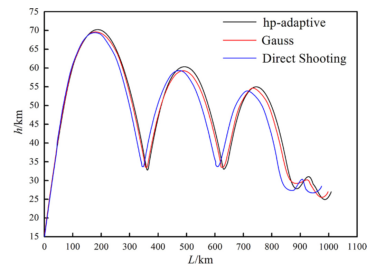
\includegraphics[width=0.7\linewidth]{figures/2_literature-review/OptimisationMethodComparisonChai}
\caption{}
\label{fig:OptimisationMethodComparisonChai}
\end{figure}


These results indicate that the pseudospectral method does not exhibit instabilities with nonlinear effects such as atmospheric density varying the dynamics of the system being optimised, and that the pseudospectral method can be used for systems with at least up to six state variables.

Based on the proven track record of the pseudospectral method in simulation situations, it was decided that using the pseudospectral method for the optimisation of the rocket-scramjet-rocket system was a sound and feasible decision. It has been necessary to investigate the range of solvers available that will utilise a pseudospectral method to solve an optimisation problem with the desired capabilities and usability. 

\subsection{Available Solvers}
\textcolor{red}{change this section to reflect more current perspective}

The pseudospectral method has a number of solvers available commercially, the foremost of which are DIDO, produced by Elissar Global \cite{Ross2002}, GPOPS II \cite{Rao2010} and PROPT, a module integrated with TOMLAB \cite{Rutquist2010}. These solvers utilise nonlinear programming techniques to solve optimal control problems in discretised form and are all similar in their operation. These have been investigated for a variety of considerations with details available in Section \ref{Achievements to Date}. 

There are a number of existing programs that can complete optimisation problems using the pseudospectral method and as such creating an optimiser from scratch was considered to be overly time consuming and not a useful contribution. A number of programs were found, which are detailed in Table \ref{table:programs}.
\begin{table}[!ht]
	
	\begin{tabular}{|c|c|c| p{7cm}|}
		\hline \textbf{Software} & \textbf{Platform} & \textbf{Cost} & \textbf{Notes} \\ 
		\hline DIDO & MATLAB & \$50 (Student) & Simple and automated with free trial available. Documentation readily available. Can perform required problem. Provides costates and Hamiltonian values.\\ 
		\hline GPOPS II & MATLAB & \$100 & Free trial available, but was unable to obtain. Some documentation available. Can perform required problem.\\ 
		\hline ROC-HJ Solver & C++ & Free & A basic solver for some specific optimal control problems. Does not perform collocation. \\ 
		\hline PROPT (IPOPT) & MATLAB & \$500 & No free trial. Documentation available. Can perform required problem. \\ 
		\hline Imperial College OCS & MATLAB & Free & Documentation and download unavailable \\ 
		\hline PSOPT & C++ & Free & Open source and can perform required problem. Not updated, many modules out of date. \\ 
		\hline 
	\end{tabular} 
	
	\caption{Summary of programs capable of pseudospectral optimisation.}
	\label{table:programs}
\end{table}
An effort was made to find an open source program that could complete the desired optimisation however it was found that all open source programs studied were out of date or not well supported. Out of the premium packages available GPOPS II and DIDO were considered the best options, both being proven in aerospace applications, with available free trials and affordable price points. Free trials were requested from both, however the free trial for GPOPS II was not received while the free trial for DIDO was received with good customer service provided. On reception of the DIDO trial it was found that DIDO provides the required optimiser package in an easy to use form, with sufficient documentation and examples provided to streamline the simulation process. DIDO also provides costate and Hamiltonian values, used for verifying that the optimised solution is accurate and physically sound, as well as the lowest price point and benefit of being proven in both real space applications and in-atmosphere simulations. After weighing these considerations DIDO was selected as the best program to use for the pseudospectral optimisation and simulation. 

\section{Aerodynamic Analysis}
- preliminary design requires fast and easy aerodynamics 

Simulating the trajectory of access to space vehicles requires the aerodynamics of the launch vehicle to be characterised accurately. This entails the creation of large aerodynamic coefficient databases, which cover the operable region of the vehicle, and include the effect of control surface deflections. The liability of the vehicle design to change during the preliminary design phases renders highly accurate CFD or experimental studies expensive and inefficient CITATION. Instead, solutions are found which are able to approximate the aerodynamic characteristics to an appropriate accuracy, while providing fast set-up speeds as well as computation times. 

\subsection{HYPAERO}

Hypaero is an aerodynamic calculation tool developed for the preliminary design of hypersonic vehicles. 
HYPAERO uses strip theory, dividing the surface of the vehicle into panels to calculate aerodynamic properties along the aircraft as illustrated in Figure \ref{fig:strip}. In strip theory two dimensional sections are created running the length of the vehicle, defining streamlines along the vehicle faces. Pressure, Mach number and skin friction are calculated along these streamlines to compute the aerodynamic coefficients of the vehicle. The Aerodynamic analysis of the SPARTAN has been performed using HYPAERO by Jazra et al. \cite{Jazra2013}. The aerodynamic coefficients of the SPARTAN vehicle have been provided for this study by Dawid Preller.

\textcolor{red}{NEED TO CHANGE THIS to clarify where I'm using this}

\begin{figure}[ht]
	\centering
	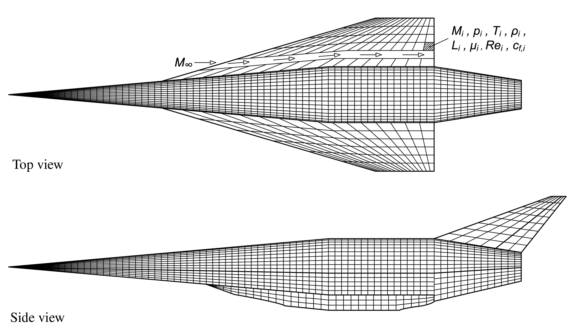
\includegraphics[width=0.7\linewidth]{strip}
	\caption{HYPAERO analysis surface grid \cite{Jazra2013}.}
	\label{fig:strip}
\end{figure}

\begin{figure}
\centering
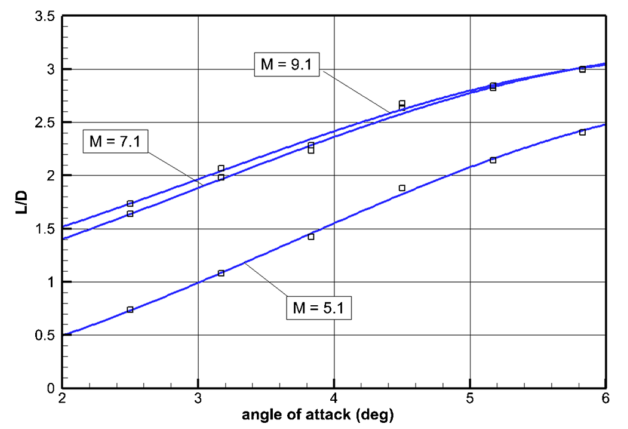
\includegraphics[width=0.7\linewidth]{figures/2_literature-review/HYPAERO-aero}
\caption{SPARTAN aerodynamics, developed using HYPAERO \cite{Preller2017}.}
\label{fig:HYPAERO-aero}
\end{figure}


\subsection{CART3D}
CART3D is an inviscid CFD package, designed for use during preliminary vehicle design and analysis CITATION. CART3D requires only a surface triangulation of the vehicle being analysed. CART3D features adjoint mesh adaption, and uses cartesian 'cut-cells' which intersect the surface, allowing complex geometries to be analysed. The mesh automatically refines as the simulation progresses, reducing error. The absence of a requirement for a user generated mesh allows CART3D to be easily applied to complex launch vehicle designs, as well as allowing for simple modification of control surface deflections and flight conditions. 
CART3D has been used extensively for aerodynamic simulations in preliminary design, including analysis of the Skylon spaceplane\cite{Mehta2016}, HIFiRE-5\cite{Kimmel2010}, and in low sonic boom shape optimisations\cite{Aftosmis2011}. 
Mehta et al. used CART3D to analyse the Skylon spaceplane, in a study which investigated the aerodynamics of the vehicle as well as the plumes produced by the Reaction Engines LTD SABRE engines\cite{Mehta2016}. The Skylon was analysed at a range of mach numbers from 2.625 to 16.969, at altitudes from 15.326km to 75.771km. These results indicate the applicability of CART3D over a wide range of Mach numbers, which is of particular use to this study.
\begin{figure}
\centering
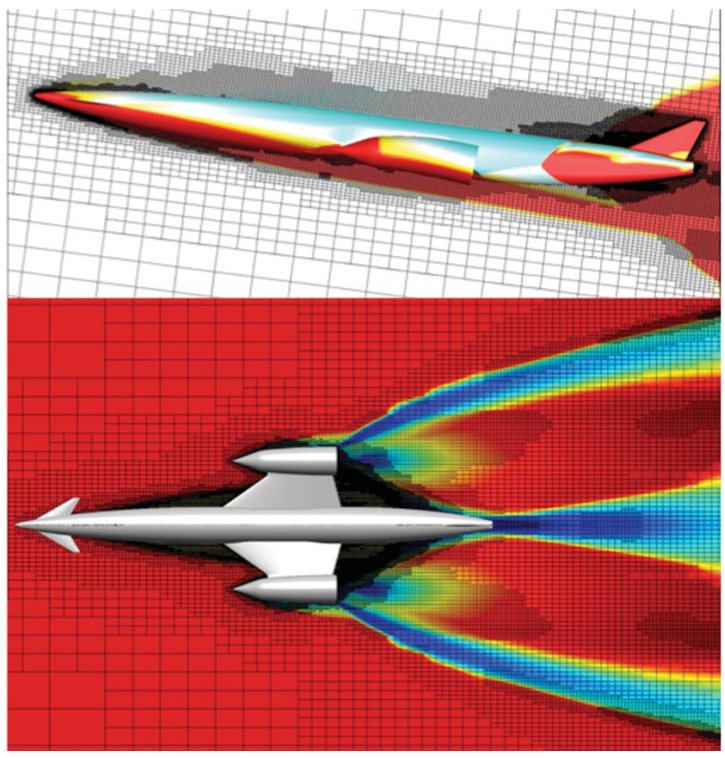
\includegraphics[width=0.6\linewidth]{figures/2_literature-review/Skylon-CART3D}
\caption{The Skylon spaceplane, simulated using CART3D at Mach 12.189, $\alpha=7.512^\circ$\cite{Mehta2016}. Cell distribution produced by mesh adaption is shown.}
\label{fig:Skylon-CART3D}
\end{figure}
During a study by Aftosmis \& Nemec where CART3D was applied to low sonic boom shape optimisation, CART3D was shown to have good agreement with experimental results in tests at Mach 1.6. 

The wide Mach number range of CART3D, along with its ease of use and demonstrated accuracy, makes CART3D a useful tool for this study. 

\subsection{Missile DATCOM}
Missile DATCOM is a widely used, semi-empirical, aerodynamic prediction tool for missile configurations. Missile DATCOM is capable of calculating the aerodynamic forces, stability derivatives and moments over a range of angle of attack and Mach number values, allowing an aerodynamic database to be generated simply and rapidly. Missile DATCOM has been shown to produce close agreement with experimental wind tunnel data for normal force and pitching moment coefficients, and reasonable agreement for axial force coefficients \cite{Sooy2005}. 

  \section{Summary}\label{chapter2:summary}

      This chapter has reviewed literature relevant to this thesis. Add more details.
      
      
      
      
